\documentclass[serif,9pt]{beamer}
\usetheme{tree}
%\usepackage{german}
\usepackage[latin1]{inputenc}
\usepackage[spanish]{babel}

% Images
\usepackage{graphicx}
\usepackage{subfigure} % subfiguras
\usepackage{caption}
\usepackage{float}
\captionsetup[table]{labelformat=empty}
\captionsetup[figure]{labelformat=empty}

\usepackage{amsmath}

\begin{document}

\title{Pr�ctica 1: An�lisis de Eficiencia de Algoritmos}  
\author{Patricia C�rdoba Hidalgo \\ Inmaculada Mar�n Carballo \\
Emilio Jos� Hoyo Medina \\ David Cabezas Berrido}
\date{}

\begin{frame}
\titlepage
\end{frame}

\begin{frame}\frametitle{�ndice}\tableofcontents
\end{frame} 

\section{Eficiencia Te�rica}

\subsection{Algoritmos de orden de eficiencia $O(n^2)$}

\begin{frame}[fragile]\frametitle{Selecci�n}
\begin{verbatim}
    1  static void seleccion_lims(int T[], int inicial, int final)
    2  {
    3    int i, j, indice_menor;
    4    int menor, aux;
    5    for (i = inicial; i < final - 1; i++) {
    6      indice_menor = i;
    7      menor = T[i];
    8      for (j = i; j < final; j++)
    9      if (T[j] < menor) {
   10        indice_menor = j;
   11        menor = T[j];
   12      }
   13      aux = T[i];
   14      T[i] = T[indice_menor];
   15      T[indice_menor] = aux;
   16    };
   17  }
\end{verbatim}
\end{frame}

\begin{frame}\frametitle{Selecci�n}
\begin{equation*}
  \sum\limits_{i=0}^{n-2}\left(\left(\sum\limits_{j=i}^{n-1}a\right)+b\right) = \sum\limits_{i=0}^{n-2}\sum\limits_{j=i}^{n-1}a + \sum\limits_{i=0}^{n-2}b
\end{equation*}

\begin{flushleft}
  $a$ acota el cuerpo del bucle interno y $b$ las asignaciones del
  cuerpo del externo.
\end{flushleft}

\text{Primer sumando (cuadr�tico)}
\begin{align*}
  \sum\limits_{i=0}^{n-2}\sum\limits_{j=i}^{n-1}a
  &=\sum\limits_{i=0}^{n-2}a(n-i)=
  \sum\limits_{i=0}^{n-2}an - \sum\limits_{i=0}^{n-2}ai \\
  &= an(n-1)-a\frac{(n-2)(n-1)}{2} \\
  &= \frac{a}{2}n^2-\frac{5a}{2}n-a \in O(n^2)
\end{align*}
\end{frame}

\begin{frame}\frametitle{Selecci�n}
\text{Segundo sumando (lineal)}
\begin{equation*}    
\sum\limits_{i=0}^{n-2}b=b\sum\limits_{i=0}^{n-2}1=b(n-1) \in O(n)
\end{equation*}

\vspace{10mm}
\begin{flushleft}
Eficiencia resultante: $\text{max}\{O(n^2), O(n)\} = O(n^2)$ 
\end{flushleft}
\end{frame}

\subsection{Algoritmos de orden de eficiencia $O(n\log n)$}

\begin{frame}[fragile]\frametitle{Heapsort: reajustar}
\begin{verbatim}
    1  static void reajustar(int T[], int num_elem, int k)
    2  {
    3    int j;
    4    int v;
    5    v = T[k];
    6    bool esAPO = false;
    7    while ((k < num_elem/2) && !esAPO)
    8    {
    9      j = k + k + 1;
   10      if ((j < (num_elem - 1)) && (T[j] < T[j+1]))
   11        j++;
   12      if (v >= T[j])
   13        esAPO = true;
   14      T[k] = T[j];
   15      k = j;
   16    }
   17    T[k] = v;
   18  }
\end{verbatim}
\end{frame}

\begin{frame}\frametitle{Heapsort: reajustar}
\begin{flushleft}
  Peor caso: $k = 0$
  
  \vspace{10mm}
  
  $k$ se duplica en cada iteraci�n (despreciando el $+1$).

\vspace{10mm}
  
  El bucle \texttt{while} se ejecutar� $\log_2 \frac{n}{2}$ veces donde $n$ es
  el tama�o del vector (num\_elem).

  \vspace{10mm}

  El cuerpo del bucle tiene eficiencia constante, lo acotamos por $a$
  y nos queda que la eficiencia de esta funci�n es $a\log_2 \frac{n}{2} \in O(\log n)$
\end{flushleft}
\end{frame}

\begin{frame}[fragile]\frametitle{Heapsort}
\begin{verbatim}
    1  static void heapsort(int T[], int num_elem)
    2  {
    3    int i;
    4    for (i = num_elem/2; i >= 0; i--)
    5      reajustar(T, num_elem, i);
    6    for (i = num_elem - 1; i >= 1; i--)
    7      {
    8        int aux = T[0];
    9        T[0] = T[i];
   10        T[i] = aux;
   11        reajustar(T, i, 0);
   12      }
   13  }
\end{verbatim}
\end{frame}
 
\begin{frame}\frametitle{Heapsort}
\begin{flushleft}
  El primer bucle se ejecuta $\frac{n}{2}+1$ veces.

  \vspace{4mm}
  
  La funci�n reajustar tiene eficiencia logar�tmica, se puede
  acotar por $a\log n$, siendo $a$ constante y $n$ el
  n�mero de elementos.

  \vspace{4mm}

  La eficiencia del primer bucle ser�a
  $a(\frac{n}{2}+1)\log n \in O(n\log n)$.

  \vspace{4mm}

  El segundo bucle se ejecuta $n-1$ veces. La eficiencia de las l�neas
  8, 9 y 10 se pueden acotar por una constante $b$.

  \vspace{4mm}

  La eficiencia del segundo bucle ser�a
  $(n-1)(a\log n + b) \in O(n\log n)$.

  \vspace{4mm}

  Eficiencia del algoritmo: $O(n\log n)$.
  
\end{flushleft}
\end{frame}

\subsection{Algoritmos de orden de eficiencia $O(n^3)$: Floyd}
\begin{frame}[fragile]\frametitle{Floyd}
  \begin{verbatim}
    1  void Floyd(int **M, int dim)
    2  {
    3    for (int k = 0; k < dim; k++)
    4    for (int i = 0; i < dim;i++)
    5    for (int j = 0; j < dim;j++)
    6    {
    7      int sum = M[i][k] + M[k][j];    	
    8      M[i][j] = (M[i][j] > sum) ? sum : M[i][j];
    9    }
    10  }
  \end{verbatim}
\end{frame}

\begin{frame}\frametitle{Floyd}

  $a$ = Constante que acota el cuerpo del tercer bucle (l�neas 7 y 8)

  $$\sum\limits_{k=0}^n\sum\limits_{i=o}^n\sum\limits_{j=0}^na=an^3$$
  Eficiencia: $O(n^3)$
\end{frame}

\subsection{Algoritmos de orden de eficiencia $O(2^n)$: Hanoi}
\begin{frame}[fragile]\frametitle{Hanoi}
\begin{verbatim}
    1  void hanoi (int M, int i, int j)
    2  {
    3    if (M > 0)
    4    {
    5       hanoi(M-1, i, 6-i-j);
    6       cout << i << " -> " << j << endl;
    7       hanoi (M-1, 6-i-j, j);
    8    }
    9  }
\end{verbatim}
\end{frame}

\begin{frame}\frametitle{Hanoi}

  Ecuaci�n en recurrencia:
  \[T(M) = T(M-1) + a + T(M-1) = 2T(M-1)+a\]

  Ecuaci�n caracter�stica:
  \[(x-2)(x-1) = 0\]

  Soluci�n:
  \[T(M) = c_12^M+c_2\]

  Eficiencia: $O(2^n)$
\end{frame}

\section{Eficiencia Emp�rica}

\subsection{Ordenaci�n $O(n^2)$}

\subsubsection{Burbuja}
\begin{frame}\frametitle{Burbuja}
\begin{figure}[H]
\centering
\subfigure[Burbuja]{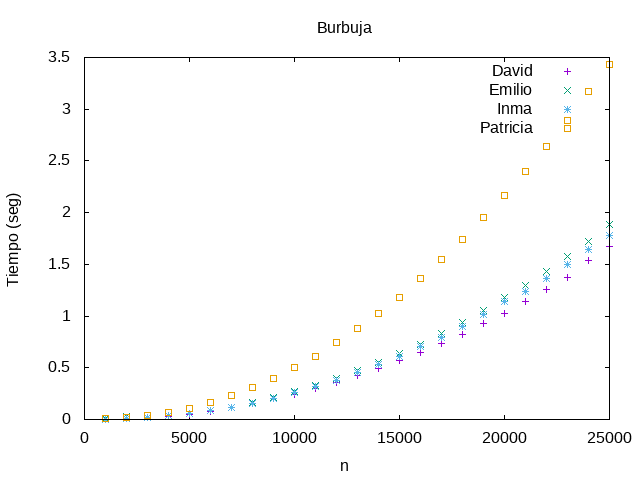
\includegraphics[width=90mm]{grupo/burbuja}}
\end{figure}
\end{frame}

\subsubsection{Inserci�n}
\begin{frame}\frametitle{Inserci�n}
\begin{figure}[H]
\centering
\subfigure[Inserci�n]{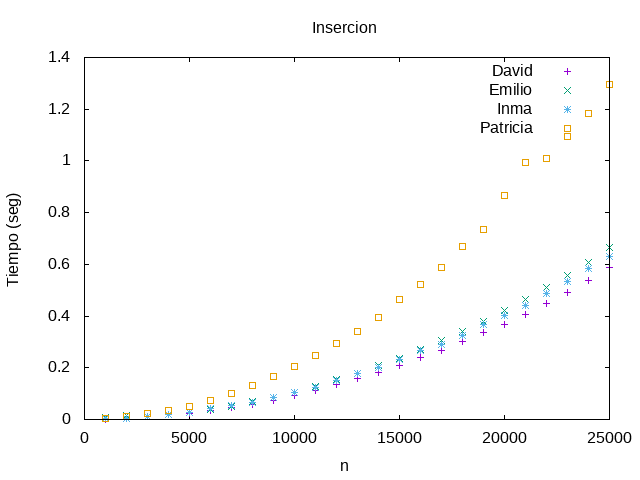
\includegraphics[width=90mm]{grupo/insercion}}
\end{figure}
\end{frame}

\subsubsection{Selecci�n}
\begin{frame}\frametitle{Selecci�n}
\begin{figure}[H]
\centering
\subfigure[Selecci�n]{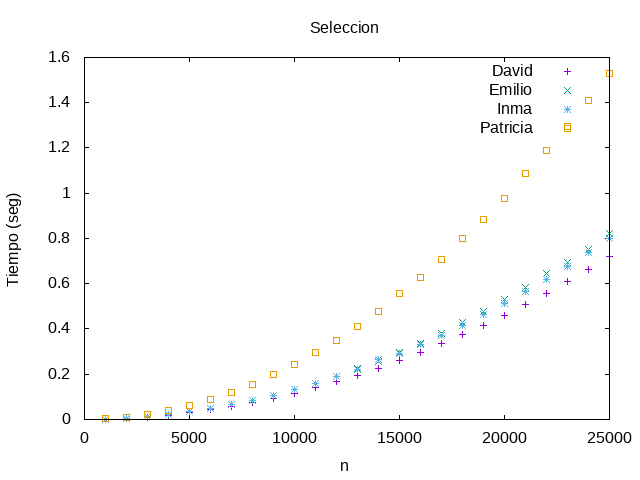
\includegraphics[width=90mm]{grupo/seleccion}}
\end{figure}
\end{frame}

\subsection{Ordenaci�n $O(n\log n)$}
  
\subsubsection{Quicksort}
\begin{frame}\frametitle{Quicksort}
\begin{figure}[H]
\centering
\subfigure[Quicksort]{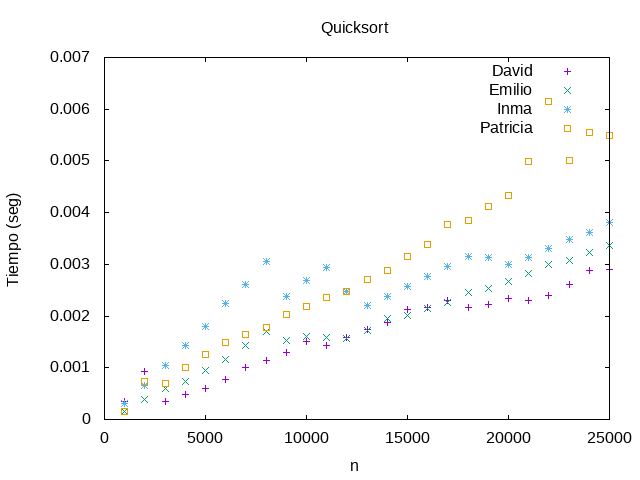
\includegraphics[width=90mm]{grupo/quicksort}}
\end{figure}
\end{frame}

\subsubsection{Mergesort}
\begin{frame}\frametitle{Mergesort}
\begin{figure}[H]
\centering
\subfigure[Mergesort]{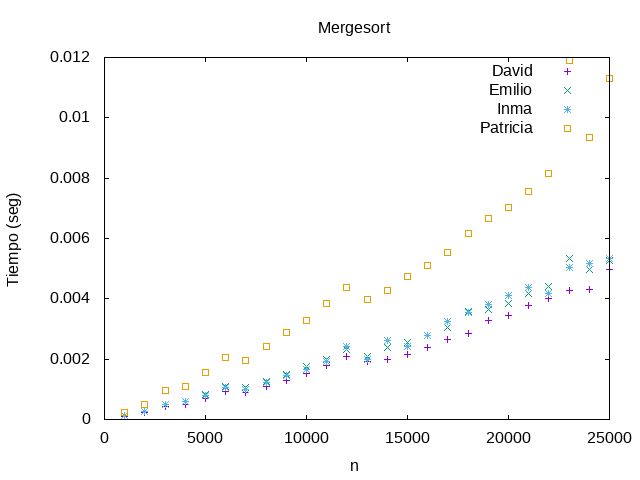
\includegraphics[width=90mm]{grupo/mergesort}}
\end{figure}
\end{frame}

\subsubsection{Heapsort}
\begin{frame}\frametitle{Heapsort}
\begin{figure}[H]
\centering
\subfigure[Heapsort]{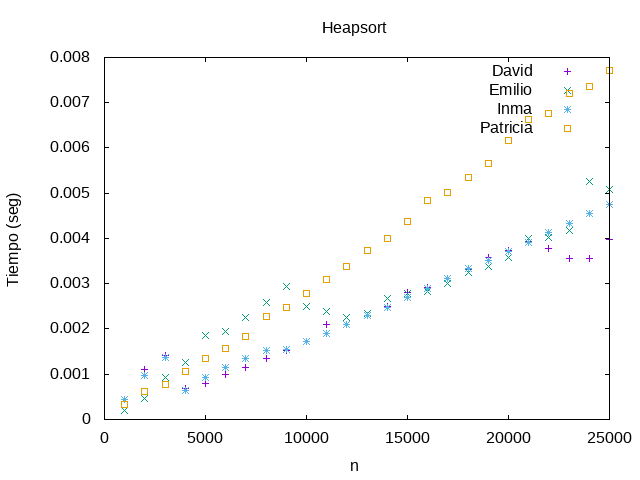
\includegraphics[width=90mm]{grupo/heapsort}}
\end{figure}
\end{frame}

\subsection{$O(n^3)$: Floyd}
\begin{frame}\frametitle{Floyd}
\begin{figure}[H]
\centering
\subfigure[Floyd]{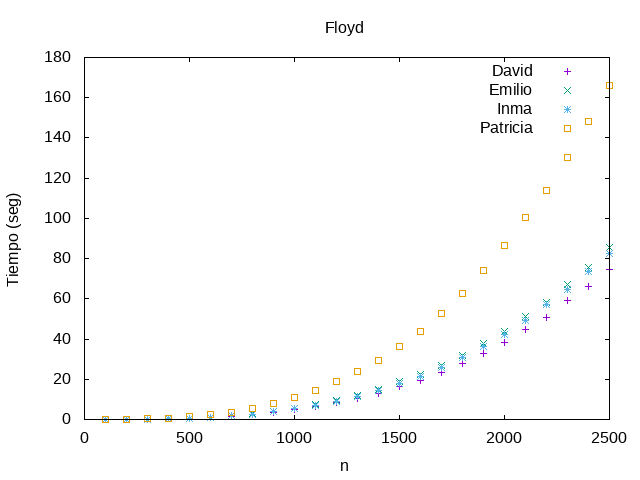
\includegraphics[width=90mm]{grupo/floyd}}
\end{figure}
\end{frame}

\subsection{$O(2^n)$: Hanoi}
\begin{frame}\frametitle{Hanoi}
\begin{figure}[H]
\centering
\subfigure[Hanoi]{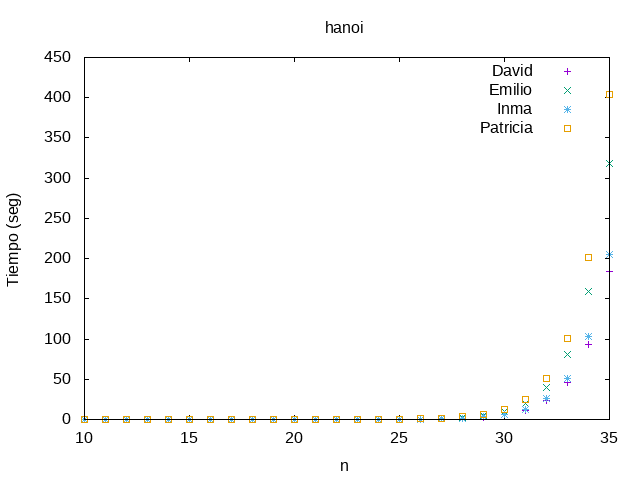
\includegraphics[width=95mm]{grupo/hanoi}}
\end{figure}
\end{frame}

\end{document}